\documentclass[12pt]{article}
\usepackage{amssymb,amsfonts,amsmath,mathtext,mathtools}
\usepackage{xfrac}
\usepackage{url, hyperref}
\usepackage[inline, shortlabels]{enumitem}


\newcommand{\avg}[1]{\langle{#1}\rangle}
\newcommand{\W}{\Omega}
\newcommand{\w}{\omega}
\newcommand{\nbar}{\bar n}
\newcommand{\rd}{\mathrm{d}}
\newcommand{\ddt}[1]{\frac{\rd{#1}}{\rd t}}
\newcommand{\D}{\Delta}
\newcommand{\geff}{\gamma_{eff}}

\title{Frequency Domain Method}

\begin{document}
	\maketitle
	\begin{abstract}
		A new method for searching for the electric dipole moment (EDM) of the deuteron and other nuclei is presented. When trying to measure the EDM in a storage ring environment, magnetic dipole moment (MDM) spin precession due to machine imperfections becomes the primary source of systematic error. The proposed method aims at providing a solution to the machine imperfection problem. The method is based on estimating the combined MDM + EDM spin precession angular velocity, in which the MDM contribution is due only to field imperfections. The MDM term is canceled in the final statistic by  adding angular velocity estimates from cycles with counter-circulating beams. Spin precession rate depends on the particle's effective Lorentz factor; the proposed method's core feature is a procedure for equalizing the effective Lorentz factors of the clockwise and counter-clockwise circulating beams, thus enabling the cancelation.
	\end{abstract}

\tableofcontents

\section{Introduction}

\section{Machine imperfection MDM spin precession}
Tilting of the accelerator optical elements about the beam axis induces a non-zero average radial magnetic field, which causes an EDM-faking MDM precession. 

We have simulated the machine imperfection precession rate $\W_{MDM}$ for the frozen spin lattice depicted in Figure~\ref{fig:Lattice}. The lattice utilizes cylindrical E+B field spin rotators in the arc sections in order to effect the frozen spin condition. Imperfections were simulated via rotations of the E+B elements about the optical axis by normally-distributed angles $\Theta_{tilt}\sim N(0,10^{-4})$~rad. The standard deviation of $10^{-4}$~rad was chosen as an estimate of a practically-achievable element alignment error level. Analytical estimates~\cite{Senichev:FDM} show, that at this level, the machine imperfection $\W_{MDM}$ should be expected in the range of 50 to 100 rad/sec, assuming an $n=100$ element lattice.

\begin{figure}[h]\centering
	\includegraphics[width=\linewidth]{Figures/BNL}
	\caption{Frozen spin lattice with cylindrical E+B field spin rotators inserted into the arc sections.\label{fig:Lattice}}
\end{figure}

Simulation results are presented in Figure~\ref{fig:MDM_vs_tilt}. One can observe that at $\avg{\Theta_{tilt}}=10^{-4}$~rad the radial component of $\W_{MDM}$ is approximately 500~rad/sec. 
Since $\sigma[\avg{\Theta_{tilt}}]~=~\sigma[\Theta_{tilt}]/\sqrt{n} = 10^{-4}/\sqrt{100} = 10^{-5}$~rad. The dependence in Figure~\ref{fig:MDM_vs_tilt} is linear, hence the probability of observing $\W_{MDM}\le 50$~rad/sec is 68\%, $\W_{MDM}\le 100$~rad/sec is 95\%, and $50\le\W_{MDM}\le100$~rad/sec with a 27\% probability.

\begin{figure}[h]\centering
	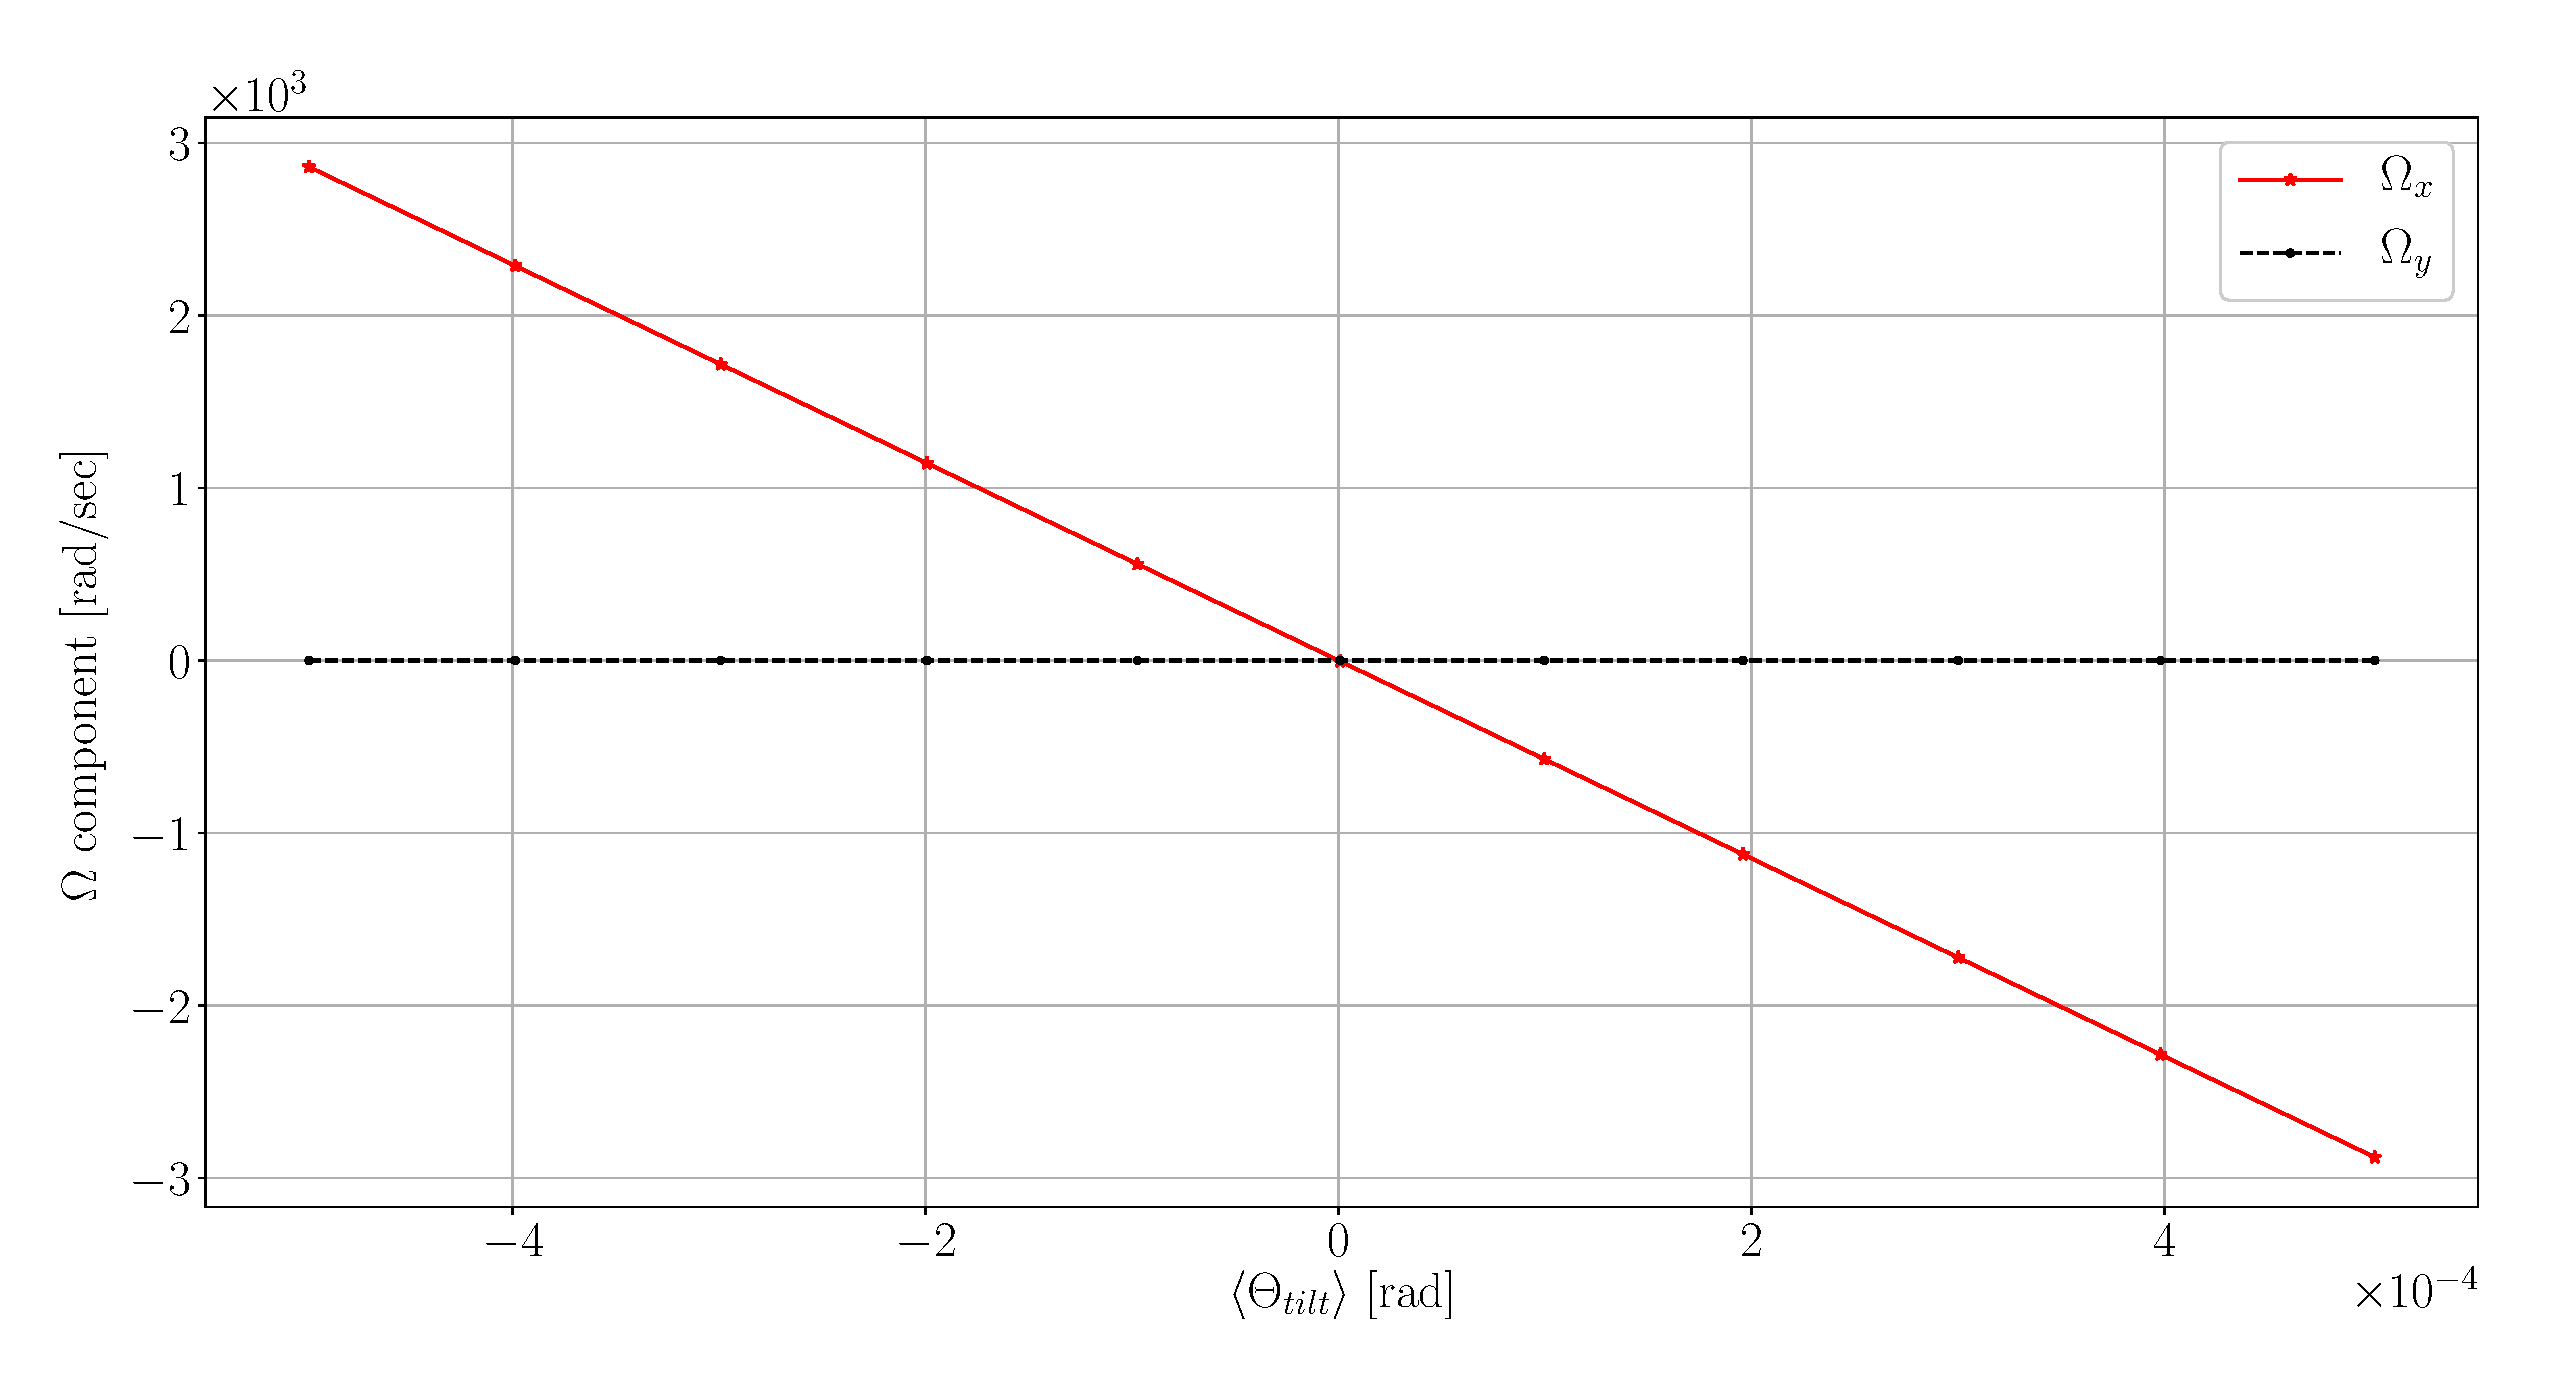
\includegraphics[width=\linewidth]{Figures/linearity_test_shifting_gauss_freq}
	\caption{Spin precession angular velocity components vs mean E+B element tilt angle.\label{fig:MDM_vs_tilt}}
\end{figure}

%\section{Spin Wheel}
%
%\subsection{Critique of the SW method}
%The Spin Wheel method is based on two equations:
%\begin{align}
%	\avg{\Omega_V}_x &= -\frac{Ze}{\gamma Am_pc}\left(\avg{B_x} - \frac{\avg{E_z}}{\beta}\right) \equiv 0, \label{eq:B-to-offset}
%	\shortintertext{and}
%	\avg{\Omega_x} &= -\frac{Ze}{Am_pc}\frac{1+a}{\gamma^2}\left(\avg{B_x} + \frac{\eta}{a}\avg{E_x}\right).\label{eq:B-to-s-prec}
%\end{align}
%Equation~\eqref{eq:B-to-offset} determines the relationship between the average radial magnetic field present in the beamline, and the resulting vertical shift of the beam's closed orbit:
%\begin{equation}
%	\avg{z} = \frac{1}{\avg{G_z}}\Big[\beta\avg{B_x} - \avg{E_z(0)}\Big].
%\end{equation}
%
%Equation~\eqref{eq:B-to-s-prec} connects the magnetic field to the beam's spin precession frequency.

\section{Frequency Domain Method}
\subsection{EDM estimator statistic}
Since the measured angular velocity $\W = \W_{MDM} + \W_{EDM}$ includes a contribution due to the MDM, one has to find a way to eliminate the $\W_{MDM}$ term from the final $\hat\W_{EDM}$ estimator. 

In the proposed methodology, non-spurious $\W_{MDM}$ is generated only by the radial magnetic fields induced by accelerator element tilts about the optical axis. Therefore, by reversing the polarity of the guide field one also reverses the sign of $\W_{MDM}$. The EDM estimator is constructed as a sum of positive (beam circulates clockwise) and negative (counter-clockwise) polarity cycles' angular momentum estimates:
\begin{align}
	\W^{\pm} &= \pm \W_{MDM} + \W_{EDM},\\
	\hat\W_{EDM} &= \frac12\left[\hat\W^+ + \hat\W^-\right] \notag\\
	&= \W_{EDM} + \frac{1}{\sqrt{2}}\cdot\sigma_{MDM} + \epsilon,	
\end{align}
where
$\sigma_{MDM}$ is  the statistical (model parameter estimate) error, and the difference between the two cycles' MDM spin precession rates $\epsilon~=~\W_{MDM}^+~-~\W_{MDM}^-$ is the  systematic error term.

\subsection{Effective Lorentz factor}
%
The number of spin revolutions per turn, spin tune $\nu_s$, depends on the particle's  equilibrium-level energy, expressed by the Lorentz factor:
\begin{align}\label{eq:spin_tune_vs_gamma}
\nu_s^B &= G\gamma, \tag{magnetic field}\\
\nu_s^E &= \frac{G+1}{\gamma} - G\gamma. \tag{electric field}
\end{align}

Not all beam particles in a bunch are characterized by the same Lorentz factor. A particle involved in betatron
motion will have a longer orbit, and as a direct consequence of the phase stability principle,
in an accelerating structure utilizing an RF cavity, its equilibrium energy level 
must increase.

Consider the reference particle. Its longitudinal dynamics is described
by the system of equations:
\begin{equation}
\begin{cases}
\ddt{}\D\varphi &= -\w_{RF}\eta\delta, \\
\ddt{}\delta &= \frac{q V_{RF}\w_{RF}}{2\pi h\beta^2E}(\sin\varphi - \sin\varphi_0).
\end{cases}
\end{equation}
In the equations above, $\D\varphi = \varphi - \varphi_0$ and
$\delta = (p-p_0)/{p_0}$ are the deviations of the particle's phase and
normalized momentum from those of the reference particle; all other symbols have their usual meanings.
%% $V_{RF}$, $\w_{RF}$ are, respectively,
%% the RF voltage and frequency; $\eta = \alpha_0 - \gamma^{-2}$ is the slip-factor,
%% where $\alpha_0$ is the momentum compaction factor defined by $\sfrac{\Delta L}{L} = \alpha_0\delta$,
%% $L$ being the orbit length; $h$ is the harmonic number; $E$ the total energy of the particle.

The solutions of this system form a family of ellipses in the $(\varphi, \delta)$-plane, all centered at the
point $(\varphi_0,\delta_0)$. However, if one considers a particle involved in betatron oscillations, and
uses a higher-order Taylor expansion of the momentum compaction factor
$\alpha = \alpha_0 + \alpha_1\delta$, the first equation of the system
transforms into:~\cite[p.~2579]{Senichev:IPAC13}
\begin{align*}
\ddt{\D\varphi} = -\w_{RF} \Bigg[\left(\frac{\Delta L}{L}\right)_\beta &+ (\alpha_0 + \gamma^{-2})\delta \Bigg.\\
&+ \Bigg.(\alpha_1 - \alpha_0\gamma^{-2} + \gamma^{-4})\delta^2\Bigg],
\end{align*}
where $(\frac{\Delta L}{L})_\beta = \frac{\pi}{2L}[\varepsilon_xQ_x + \varepsilon_yQ_y]$, is
the betatron motion-related orbit lengthening; $\varepsilon_x$ and $\varepsilon_y$ are
the horizontal and vertical beam emittances, and $Q_x$, $Q_y$ are the horizontal and vertical tunes.

The solutions of the transformed system are no longer centered at the same single point. Orbit lengthening
and momentum deviation cause an equilibrium-level momentum shift~\cite[p.~2581]{Senichev:IPAC13}
\begin{equation}\label{eq:EquLevMom_shift}
\Delta\delta_{eq} = \frac{\gamma_0^2}{\gamma_0^2\alpha_0 - 1}\left[\frac{\delta_m^2}{2}(\alpha_1 - \alpha_0\gamma^{-2} + \gamma_0^{-4}) + \left(\frac{\Delta L}{L}\right)_\beta\right],
\end{equation}
where $\delta_m$ is the amplitude of synchrotron oscillations.

We call the equilibrium energy level associated with the momentum shift~\eqref{eq:EquLevMom_shift},
the \emph{effective Lorentz factor}:
\begin{equation}\label{eq:EffectiveGamma}
\geff= \gamma_0 + \beta_0^2\gamma_0\cdot\Delta\delta_{eq},
\end{equation}
where $\gamma_0$, $\beta_0$ are the Lorentz factor and relative velocity factor of the reference particle.

In order to minimize systematic error $\epsilon$, one needs a way to keep $\W_{MDM}$ constant across multiple runs.

The obvious way of trying to precisely reproduce the guiding field is inefficient for two major reasons:
\begin{enumerate*}[(1)]
	\item standard magnetic field measurement methods do not yield sufficient precision;
	\item the lattice might not be symmetric enough, in terms of spin dynamics, with respect to reversal of the beam circulation direction.
\end{enumerate*}
Hence, we propose a different variable for calibration.

We note that the number of spin revolutions per turn (spin tune $\nu_s$) depends on the particle's  equilibrium-level energy, expressed by the Lorentz factor $\gamma$:
\begin{align}\label{eq:spin_tune_vs_gamma}
\nu_s^B &= G\gamma, \tag{magnetic field}\\
\nu_s^E &= \frac{G+1}{\gamma} - G\gamma. \tag{electric field}
\end{align}

Not all beam particles in a bunch are characterized by the same $\gamma$. A particle involved in betatron
motion will have a longer orbit, and as a direct consequence of the phase stability principle,
in an accelerating structure utilizing an RF cavity, its equilibrium energy level 
must increase.

The effective Lorentz factor is a generalization of the regular Lorentz factor accounting for betatron motion-related orbit lengthening and non-linearity of the momentum compaction factor.

It has been shown in~\cite[p.~56]{Aksentev:Thesis} that a particle's spin tune can be described by a univariate function; we associate the argument of that function with the effective Lorentz factor. Consequently, spin-vectors of two particles characterized by the same value of the effective Lorentz factor precess as the same rate.

Therefore, if the CW and CCW beam centroids' have equal $\geff$, we can expect the MDM components of the spin precession angular velocities to be equal as well.

\subsection{Calibration of the ELF}
Now the question becomes how the effective Lorentz factor can be calibrated.


\section{Statistical precision}
Spin precession angular velocity is estimated via non-linear fit of a constant-parameter harmonic function to polarization data. However, perturbations to the spin dynamics, caused by, for example, betatron motion, introduce a mismatch between the fit model and the data, and hence a model specification systematic error. This problem has been analyzed,~\cite{Aksentev:IPAC19:SMP} with the conclusion that this systematic error is negligible.

Effective duration of the measurement cycle cannot exceed three times the polarization lifetime $\tau_d$,~\cite{Stats} where $\tau_d$ is the time during which beam polarization decreases by a factor of $e$.

Simulation shows~\cite{Stats} the possibility of reaching a statistical error $\sigma[\hat\W]~=~8\cdot~10^{-7}$~rad/sec in one measurement cycle (at $\tau_d = 10^3$~sec), and $\sigma[\avg{\hat\W}]~=~5\cdot~10^{-9}$~rad/sec in one year of measurement (at 70\% accelerator time load). This should suffice to achieve an EDM estimate precision level of $10^{-29}~e\cdot$cm.

\begin{thebibliography}{0}
%	\bibitem{Senichev:IPAC13}
%	Y. Senichev et al., ``Spin tune decoherence effects in Electro- and Magnetostatic Structures.''
%	Proceedings of IPAC 2013, Shanghai, China, pp. 2579-2581.
	\bibitem{Senichev:FDM}
	Y. Senichev, A. Aksentev, A. Ivanov, E. Valetov, ``Frequency domain method of the search for
	the deuteron electric dipole moment in a storage ring with imperfections,'' arxiv:1711.06512 [physics.acc-ph]
	\url{https://arxiv.org/abs/1711.06512}.
	\bibitem{Aksentev:Thesis}
	A. Aksentev, ``2D Frozen spin method of searching for the deuteron EDM in a storage ring.'' PhD thesis, NRNU ``MEPhI,'' Moscow, Russia.
	\url{http://collaborations.fz-juelich.de/ikp/jedi/public_files/theses/dissertation.pdf}
	\bibitem{Aksentev:IPAC19:SMP}
	A. Aksentev, Y. Senichev, ``Spin Motion Perturbation Effect on the EDM Statistic
	in the Frequency Domain Method,'' presented at the 10th International Particle Accelerator Conf. (IPAC'19),
	Melbourne, Australia, May. 2019.
	\url{https://ipac2019.vrws.de/papers/mopts011.pdf}
	\bibitem{Stats}
	A.E. Aksentev, Y.V. Senichev, ``Statistical precision in charged particle EDM search in storage rings.'' J Phys: Conf Ser. \textbf{941} (2017) 012083. 
	\url{https://iopscience.iop.org/article/10.1088/1742-6596/941/1/012083}
	
\end{thebibliography}

\end{document}